\section {Results}
\label{results}

\subsection {Analysis}
Charts will now be presented. The line charts uses time (year) on the x-axis while the y-axis is either entropy or probability. A table of words in some select topics will also be presented.

\begin{figure}[center]
	\centering
	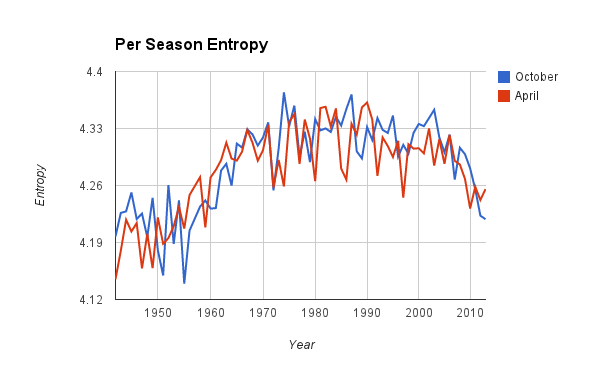
\includegraphics[width=12cm]{images/H(per-season).png}
	\caption{Per season entropy over time. The values are basically the same value according to a $t$-test.}
	\label{fig:entropy-per-season}
\end{figure}

A pair-wise t-test was computed for this series and it was found to have a \textit{p}-value of approximately $0.06$, which would generally be considered to not be statistically significant. Indeed, it appears that the April and October conferences follow each other through time in terms of entropy. This means that according to this data, hypothesis $H_2$ must be rejected.

\begin{figure}[center]
	\centering
	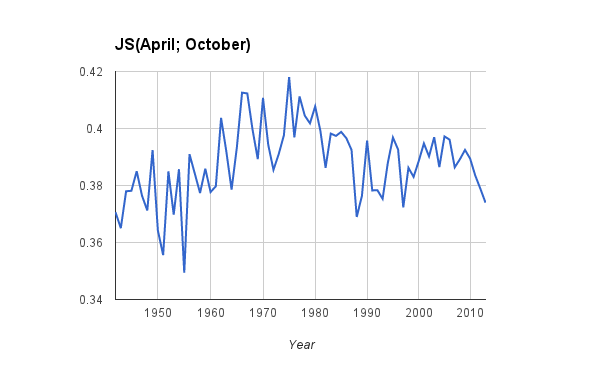
\includegraphics[width=12cm]{images/JS(April;Oct).png}
	\caption{JS divergence over time of the two seasonal venues of conference, April and October. Although not very dynamic, there are changes over time.}
	\label{fig:js-season}
\end{figure}

Although the entropy values of the two conferences are not significantly different, the topics used within the conference might vary. The Jensen-Shannon divergence value for April vs. October are charted in Figure \ref{fig:js-season}. Divergence does fluctuate from year to year, but not by much. Nevertheless, sometimes achieving a divergence value of 0.4, this divergence is greater than taht found for genders, demonstrated in Figure \ref{fig:js-gender}.

\begin{figure}[center]
	\centering
	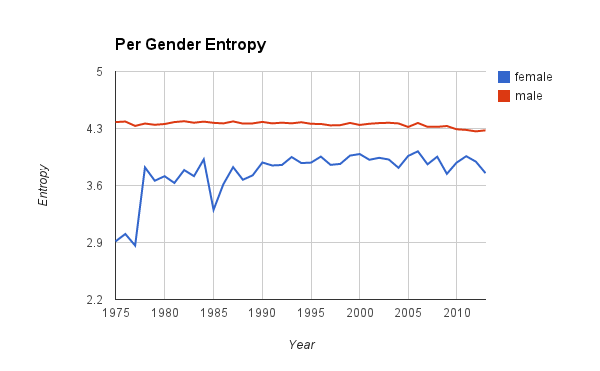
\includegraphics[width=12cm]{images/H(per-gender).png}
	\caption{Per gender entropy over time. The values are statistically significantly different according to a $t$-test.}
	\label{fig:entropy-per-gender}
\end{figure}

Again, entropy is charted over time in Figure \ref{fig:entropy-per-gender}, but this time by gender. This was found to be statistically significant ($p < 0.05$) according to a pair-wise $t$-test. It is interesting to note that although the males always have a higher entropy value, they seem to be less dynamic than females. This might be because women tend to have general positions in the church for less time than men, so they end up being more transient and therefore speak fewer times. Future work could investigate this further. Hypothesis $H_3$ is accepted.

\begin{figure}[center]
	\centering
	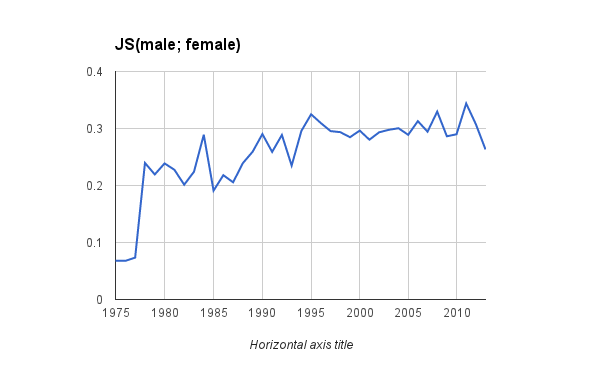
\includegraphics[width=12cm]{images/JS(female;male).png}
	\caption{JS divergence over time of the two genders, female and male. This divergence is less than that found in seasonal differences.}
	\label{fig:js-gender}
\end{figure}

The JS divergence values between topics distributions over time for each gender are found in Figure \ref{fig:js-gender}. Interestingly, the lowest points on this chart correspond to the lowest in Figure \ref{fig:entropy-per-gender}. It seems that when women started speaking in general conference, they had a lower entropy (spoke on fewer topics) and didn't differ as much from what the men were saying. 

\begin{figure}[center]
	\centering
	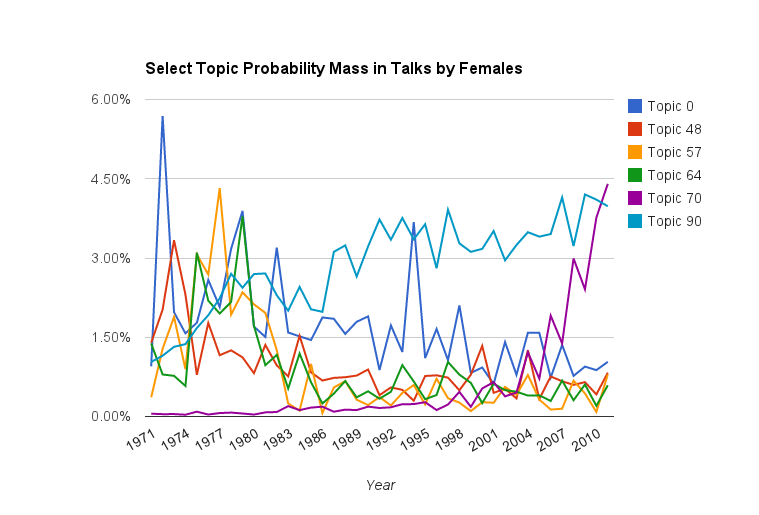
\includegraphics[width=14cm]{images/ToT(females).png}
	\caption{Probabilities of usage by females for 6 topics charted over time.}
	\label{fig:top-5-topics-ranges-female}
\end{figure}

Figures \ref{fig:top-5-topics-ranges-female} - \ref{fig:top-5-topics-ranges-male} show 5 of the  topics that had the highest range of probability of being assigned to a token in LDA. In other words. This sets them apart from other topics that are perhaps common, but do not change much. These figures support the fact that the divergences indicate that men and women are speaking on \textit{mostly} the same topics. The words that correspond to the topics in the legends for these figures is found in Table \ref{tab:select-topics} in the Appendix.

%Interestingly, %algorithm 1 is often the best algorithm. Subsequently, this is also true for the MAE over all imitation types. Algorithm 1 combined wih BP-MLP ends up being the best high-order combinational model. However, in when simple linear regression is used, algorithm 1 ends up being the worst model.

\begin{figure}[center]
	\centering
	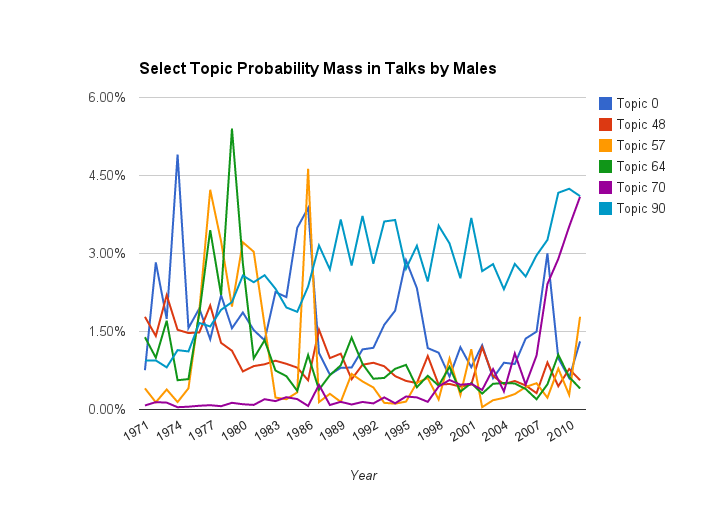
\includegraphics[width=16cm]{images/ToT(males).png}
	\caption{Probabilities of usage by males for 6 topics charted over time.}
	\label{fig:top-5-topics-ranges-male}
\end{figure}


\clearpage

%%%%%%%%%%%%%%%%%%%%%%%%%%%%%%%%%%%%
%sample helps from previous research
%%%%%%%%%%%%%%%%%%%%%%%%%%%%%%%%%%%%

%\begin{table}
	\begin{center}
		\begin{tabular}{|c|c|c|c|c|} \hline
			\textit{HOT} & \textit{BLACK} & \textit{TALL} & \textit{LARGE} & \textit{UGLY} \\ \hline \hline
			cold	&	white	&	short	&	small	&	pretty		\\
			cold	&	white	&	short	&	small	&	beautiful		\\
			cold	&	white	&	short	&	tiny	&	beautiful		\\
			cold	&	white	&	short	&	small	&	beautiful		\\
			not hot	&	not black	&	not tall	&	not large	&	not ugly		\\
			cold	&	white	&	short	&	small	&	pretty		\\
			cold	&	light	&	short	&	petite	&	pleasing		\\
			cold	&	white	&	short	&	small	&	beautiful		\\
			frigid	&	white	&	short	&	miniscule	&	breathtaking		\\
			ugly	&	white	&	short	&	small	&	pretty		\\
			cold	&	white	&	short	&	small	&	pretty		\\
			cold	&	white	&	short	&	small	&	pretty		\\
			cold	&	white	&	short	&	small	&	beautiful		\\
			cold	&	white	&	short	&	small	&	pretty		\\
			cold	&	white	&	short	&	small	&	beautiful		\\
			cold	&	white	&	short	&	small	&	pretty		\\
			cold	&	white	&	short	&	small	&	pretty		\\
			cold	&	white	&	short	&	small	&	beautiful		\\
			cold	&	white	&	short	&	small	&	Beauty 		\\
			cold	&	white	&	short	&	small	&	pretty		\\
			cold	&	white	&	short	&	small	&	beautiful		\\
			cold	&	white	&	short	&	small	&	pretty		\\
			cold	&	white	&	short	&	small	&	beautiful		\\
			cold	&	N/A	&	N/A	&	N/A	&	beautiful		\\
			cold	&	white	&	short	&	small	&	beautiful		\\
			cold	&	mirrored	&	short	&	small	&	beautiful		\\
			freezing	&	N/A	&	N/A	&	insignificant	&	N/A		\\
			cold	&	white	&	short	&	small	&	beautiful		\\
			cold	&	light	&	diminutive	&	petite	&	exquisite		\\
			cold	&	white	&	short	&	small	&	beautiful		\\
			cold	&	white	&	short	&	small	&	pretty		\\
			cold	&	white	&	short/small	&	small	&	pretty		\\
			%cold	&	white	&	short	&	small	&	beautiful		\\
			%cold	&	white	&	short	&	small	&	beautiful		\\
			cold	&	white	&	short	&	small	&	pretty		\\ \hline
			%sexless	&	white	&	short	&	diminished	&	kind		\\ 
			\textbf{6}	&	\textbf{5}	&	\textbf{5}	&	\textbf{7}	&	\textbf{8}		\\
			\hline
		\end{tabular}
	\end{center}
	\caption {All antonym responses for each adjective with total number of unique responses.}
	\label{tab:all_adjective}
\end{table}

\begin{table}
	\begin{center}
		\begin{tabular}{|c|c|c|c|c|} \hline
			\textit{ZIPPER} & \textit{SKY} & \textit{SHOE} & \textit{ROBOT} & \textit{CARPET} \\ \hline \hline
			Velcro	&	ground	&	glove	&	human	&	hard floor		\\
			button(s)	&	Earth	&	glove	&	living being	&	hard floor		\\
			Velcro	&	ground	&	sock(s)	&	Free	&	ceiling		\\
			lace(s)	&	ground	&	glove	&	human	&	ceiling		\\
			not zipper	&	not sky	&	not a shoe	&	not robot	&	not carpet		\\
			button(s)	&	ground	&	sock(s)	&	human	&	ceiling		\\
			razor	&	dirt	&	hat	&	sentient being	&	canopy		\\
			button(s)	&	ground	&	barefeet	&	human	&	tile		\\
			button(s)	&	Earth	&	barefeet	&	human	&	tile		\\
			button(s)	&	ground	&	sock(s)	&	human	&	tile		\\
			unzipper	&	ground	&	barefeet	&	organic/organism	&	ceiling		\\
			button(s)	&	Earth	&	barefeet	&	person	&	hardwood		\\
			button(s)	&	ground	&	barefeet	&	human	&	hardwood		\\
			button(s)	&	land	&	sock(s)	&	human	&	tile		\\
			button(s)	&	ground	&	sock(s)	&	organic/organism	&	tile		\\
			button(s)	&	ground	&	hat	&	human	&	wood		\\
			N/A	&	Earth	&	N/A	&	person	&	tile		\\
			button(s)	&	Earth	&	sandal	&	human	&	hardwood		\\
			Unzip	&	Earth	&	barefeet	&	human	&	hardwood		\\
			button(s)	&	ground	&	glove	&	person	&	hardwood		\\
			button(s)	&	ground	&	barefeet	&	baby	&	ceiling		\\
			ripper	&	hell	&	glove	&	human	&	hardwood		\\
			scissors	&	ground	&	hat	&	grass	&	ceiling tiles		\\
			N/A	&	N/A	&	N/A	&	rock	&	ceiling		\\
			button	&	ground	&	foot	&	human	&	air		\\
			button	&	earth	&	hat	&	ghost	&	ceiling		\\
			N/A	&	land	&	N/A	&	N/A	&	N/A		\\
			antizipper	&	ground	&	glove	&	antirobot	&	anticarpet		\\
			snaps	&	ground	&	barefeet	&	organic	&	tile		\\
			velcro 	&	floor	&	barefeet	&	human	&	tile		\\
			velcro	&	earth	&	sandal	&	human	&	wood		\\
			button(s)	&	ground	&	slipper	&	human	&	concrete		\\
			%button(s)	&	ground	&	barefeet	&	person	&	wood		\\
			%button(s)	&	ground	&	barefeet	&	human	&	wood		\\
			button(s)	&	Ground	&	hat	&	Human	&	Dirt		\\ \hline
			%zip him	&	Earth	&	barefeet	&	human	&	ambulatory pet		\\ 
			\textbf{14}	&	\textbf{8}	&	\textbf{8}	&	\textbf{13}	&	\textbf{12}		\\
			\hline
		\end{tabular}
	\end{center}
	\caption {All antonym responses for each noun with total number of unique responses.}
	\label{tab:all_noun}
\end{table}


%The Welch's \textit{t}-test agrees that there is significance (equal variance not assumed):%
%	\begin{quote}
%		$t(5)=4.1642, p < 0.00439413$
%	\end{quote}

%\subsection{}
%Since there were few responses from men (only 9), it seems that running the same \textit{t}-test on the responses without the male responses could be of interest as well.  Tables~\ref{tab:female_adjective}, \ref{tab:female_noun} show the normalized responses and total counts for each set of xyz while Table~\ref{tab:female_group_stats} shows the group statistics for the two groups.


%The calculated statistic is as follows (equal variance not assumed):
%$t(7.881)=3.55902, p < 0.00461577$ 
